% =============================================================================
% TIADC 校准技术 —— 从 Verilog ASIC 到 SoC C 语言实现
% 演示文稿 (Beamer, 16:9)
% 编译: latexmk -xelatex tiadc_cali_preso.tex
% =============================================================================
\documentclass[table,UTF8,11pt,aspectratio=169]{beamer}

% ---- 中文 ----
\usepackage{xeCJK}
\setCJKmainfont{Songti SC}
\setCJKsansfont{Heiti SC}

% ---- 主题 ----
\usetheme{Madrid}
\usecolortheme{whale}
\usefonttheme{professionalfonts}
\setbeamertemplate{navigation symbols}{}

% ---- 自定义颜色 ----
\definecolor{darkblue}{RGB}{0,51,102}
\definecolor{darkred}{RGB}{180,0,0}
\definecolor{darkgreen}{RGB}{0,120,0}
\definecolor{mygold}{RGB}{200,130,20}
\setbeamercolor{frametitle}{fg=white,bg=darkblue}

% ---- 宏包 ----
\usepackage{graphicx}
\usepackage{tikz}
\usetikzlibrary{positioning,calc,shapes.geometric,arrows.meta,fit}
\usepackage{booktabs}
\usepackage{tabularx}
\usepackage{array}
\usepackage{amsmath,amssymb}
\usepackage{listings}

\lstset{basicstyle=\tiny\ttfamily,breaklines=true,frame=single,numbers=none}

% ---- 自定义 block 样式 ----
\setbeamercolor{block title}{fg=white,bg=darkblue!80}
\setbeamercolor{block body}{fg=black,bg=darkblue!5}

\graphicspath{{./}}

% =============================================================================
\title[TIADC 校准技术]{64通道 64GSa/s TIADC 校准技术}
\subtitle{从 Verilog ASIC 到 SoC C 语言实现}
\author{GLC Knowledge Base}
\date{\today}
\institute{TIADC 校准项目组}

\begin{document}

% ===== Slide 1: 标题 =====
\begin{frame}
\titlepage
\end{frame}

% ===== Slide 2: 目录 =====
\begin{frame}{目录}
\tableofcontents
\end{frame}

% =============================================================================
\section{背景与问题}
% =============================================================================

\begin{frame}{为什么需要 TIADC？}
\begin{columns}[T]
\column{0.55\textwidth}
\begin{block}{单 ADC 的瓶颈}
\begin{itemize}
    \item \textbf{工艺限制}：CMOS 晶体管特征频率有限
    \item \textbf{功耗墙}：高速 ADC 功耗随采样率超线性增长
    \item \textbf{精度-速度矛盾}：高位宽与高速度难以兼得
\end{itemize}
\end{block}
\vspace{0.3cm}
\begin{block}{TIADC 的解决思路}
$M$ 个低速率子 ADC 并行工作：\\
每个以 $f_s/M$ 采样，相位依次错开 $1/f_s$\\
$\Rightarrow$ 等效采样率 $f_s$，为单通道的 $M$ 倍
\end{block}

\column{0.45\textwidth}
\centering
\begin{tikzpicture}[>=Latex,scale=0.7,every node/.style={font=\footnotesize}]
\node[draw,fill=blue!5] (sys) at (0,2.5) {\textbf{TIADC 系统}};
\node[draw,fill=orange!10,minimum width=1.8cm,align=center] (ch1) at (-2,0.5) {CH1\\$f_s/M$};
\node[draw,fill=orange!15,minimum width=1.8cm,align=center] (ch2) at (0,0.5) {CH2\\$f_s/M$};
\node[draw,fill=orange!20,minimum width=1.8cm,align=center] (ch3) at (2,0.5) {CH$M$\\$f_s/M$};
\draw[->] (sys) -- (ch1);
\draw[->] (sys) -- (ch2);
\draw[->] (sys) -- (ch3);
\node at (0,-0.8) {$\times M$ 采样率提升};
\node[align=center,font=\footnotesize] at (0,-1.5) {
本报告：64通道, 64 GSa/s\\
$T_s \approx 15.6$ ps};
\end{tikzpicture}
\end{columns}
\end{frame}

\begin{frame}{失配问题 —— 理想与现实的差距}
\begin{alertblock}{核心矛盾}
理论上 $M$ 个完全一致的子 ADC 能完美并行。\\
但\textbf{工艺偏差 (Process Variation)} 导致各通道不可避免的失配。\\
\textbf{不校准则 TIADC 动态性能不如单个子 ADC！}
\end{alertblock}

\vspace{0.3cm}
\begin{columns}[T]
\column{0.33\textwidth}
\begin{block}{失调失配 (Offset)}
$y_k = x_k + O_k$\\
加法性误差\\
与输入频率无关
\end{block}

\column{0.33\textwidth}
\begin{block}{增益失配 (Gain)}
$y_k = (1+\Delta G_k) x_k$\\
乘法性误差\\
与信号幅度成正比
\end{block}

\column{0.33\textwidth}
\begin{block}{时钟偏斜 (Timing Skew)}
$\epsilon \propto f_{in} \cdot \Delta t$\\
\textbf{正比于输入频率}\\
高频时影响最大！
\end{block}
\end{columns}

\vspace{0.3cm}
\centering
三种失配均在 $f_s/M$ 整数倍处引入杂散 $\rightarrow$ 严重劣化 SFDR / SNR
\end{frame}

\begin{frame}{三种失配对比总结}
\begin{table}
\rowcolors{2}{blue!5}{white}
\begin{tabular}{p{1.8cm}p{2.5cm}p{2.5cm}p{2.5cm}}
\toprule
\textbf{特性} & \textbf{Offset} & \textbf{Gain} & \textbf{Timing Skew} \\
\midrule
物理根源 & 偏置电压不匹配 & 参考电压/器件不匹配 & 时钟分配不匹配 \\
数学形式 & 加法 $+O_k$ & 乘法 $\times G_k$ & 时间位移 $\Delta t_k$ \\
频谱位置 & $f_s/M$ 整数倍 & $f_s/M$ 整数倍 & $f_s/M$ 整数倍 \\
频率关系 & 无关 & $\propto$ 信号幅度 & $\propto$ 信号频率 \\
校准难度 & $\star\star$ & $\star\star$ & $\star\star\star$ \\
校准顺序 & \textbf{第1步} & \textbf{第2步} & \textbf{第3步} \\
\bottomrule
\end{tabular}
\end{table}
\end{frame}

% =============================================================================
\section{三步校准算法}
% =============================================================================

\begin{frame}{第一步：Offset 校准 —— 指数平均法}
\begin{columns}[T]
\column{0.45\textwidth}
\begin{block}{核心公式（一阶 IIR 低通）}
$\bar{x}(n) = \bar{x}(n-1) + \alpha [x(n) - \bar{x}(n-1)]$
\end{block}
\begin{itemize}
    \item 每次采样都更新，输出连续
    \item 硬件：加法器 + 移位寄存器，无需乘法器
    \item $\alpha = 2^{-10} \sim 2^{-21}$（8档自动切换）
\end{itemize}

\column{0.55\textwidth}
\centering
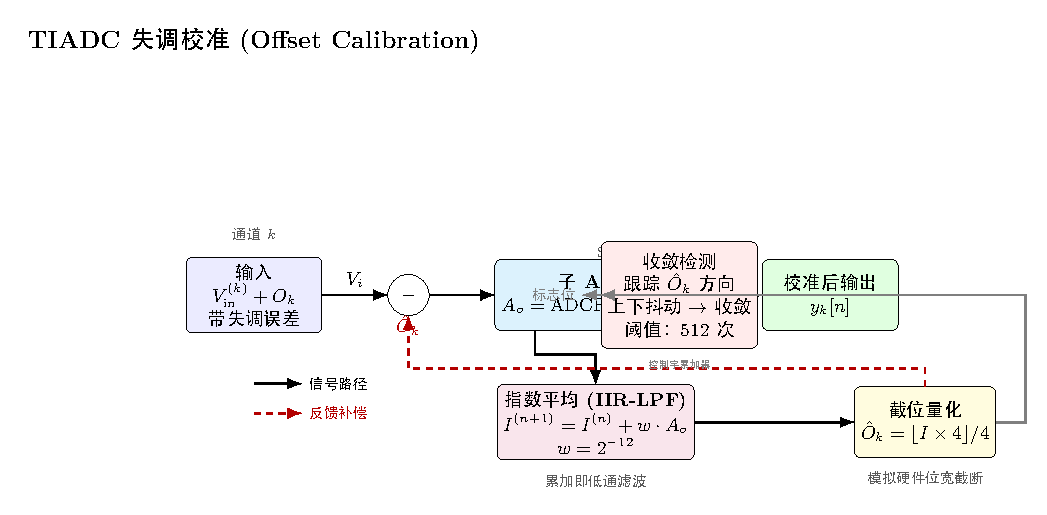
\includegraphics[width=\textwidth]{offset_cali.pdf}
\end{columns}
\end{frame}

\begin{frame}{第二步：Gain 校准 —— LMS 功率均衡}
\begin{columns}[T]
\column{0.45\textwidth}
\begin{block}{LMS 迭代公式}
$g'_i[n+1] = g'_i[n] + \alpha (T_h - y_i^2[n])$
\end{block}
\begin{itemize}
    \item 目标：消除\textbf{通道间相对增益误差}
    \item 比较各通道功率与参考功率
    \item 参考值可选：通道1功率 / 所有通道均值
    \item $\alpha = 2^{-32} \sim 2^{-39}$（极精细步长）
\end{itemize}

\column{0.55\textwidth}
\centering
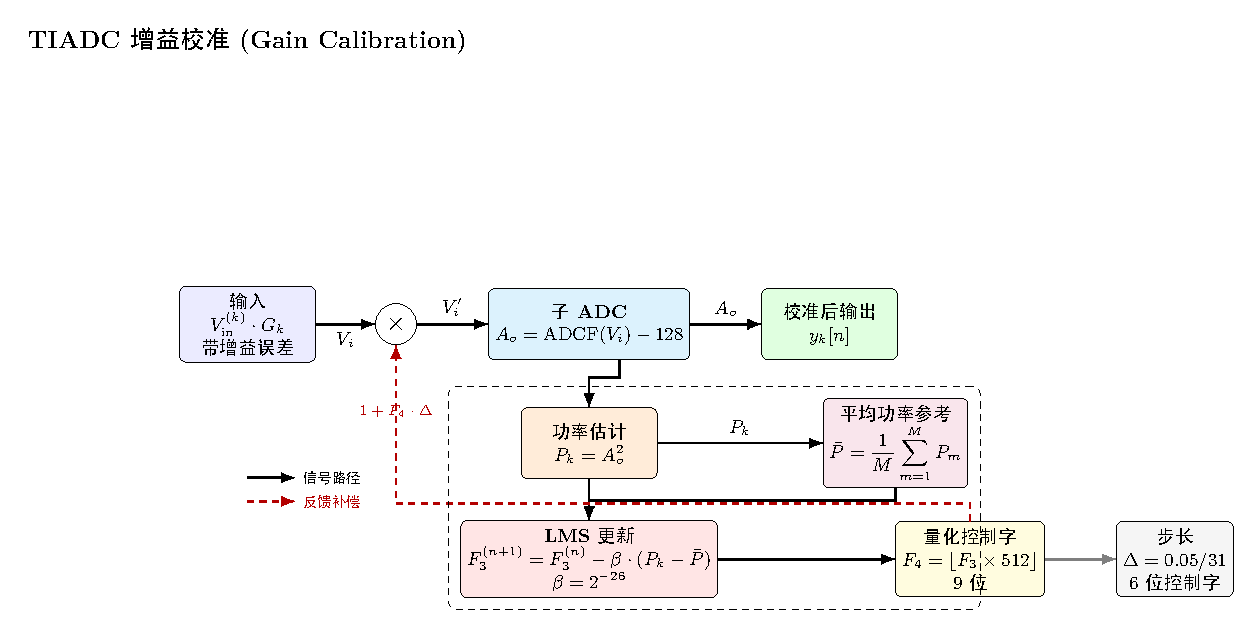
\includegraphics[width=\textwidth]{gain_cali.pdf}
\end{columns}
\end{frame}

\begin{frame}{第三步：Timing Skew 校准 —— 自相关法}
\begin{columns}[T]
\column{0.38\textwidth}
\begin{block}{自相关差值}
$D_{\Delta t} = R_x(T_{ck}-\Delta T) - R_x(T_{ck}+\Delta T)$
\end{block}
\begin{itemize}
    \item 利用相邻通道采样的互相关
    \item $D_{\Delta t}$ 符号 $\rightarrow$ 偏移方向
    \item $D_{\Delta t}$ 大小 $\rightarrow$ 偏移程度
    \item 64通道 $\rightarrow$ 4组时钟, 校准3个参数
\end{itemize}

\column{0.62\textwidth}
\centering
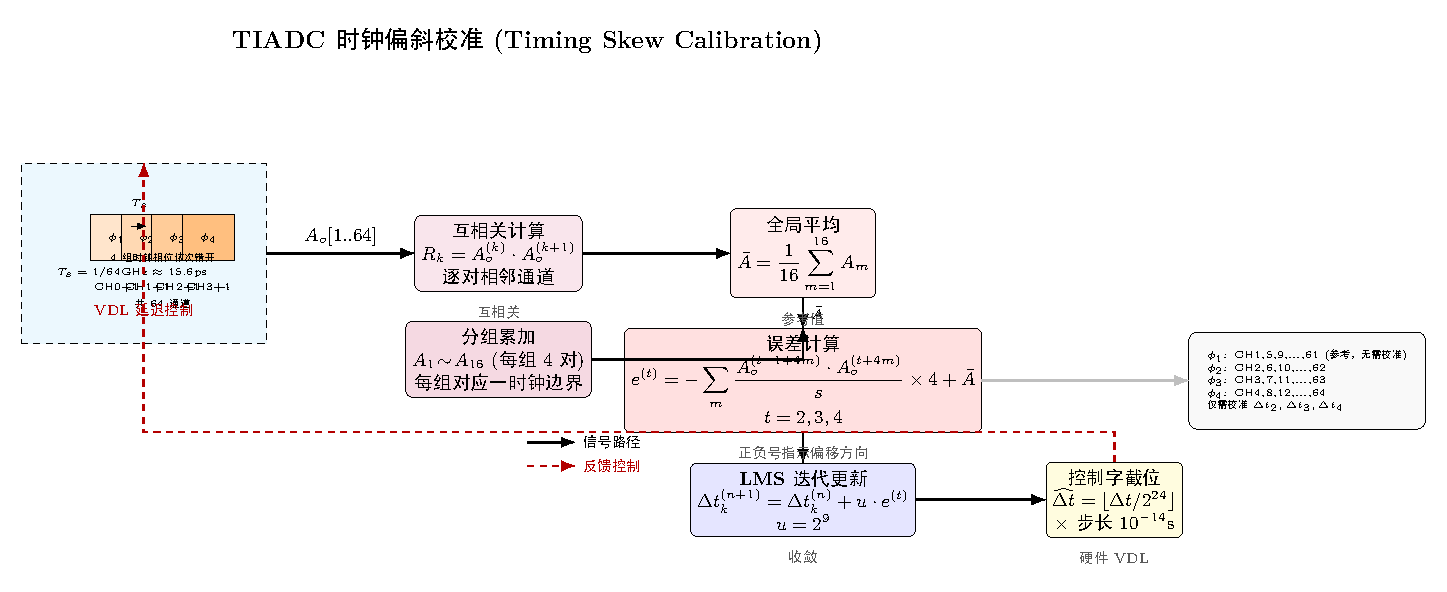
\includegraphics[width=\textwidth]{timing_cali.pdf}
\end{columns}
\end{frame}

\begin{frame}{综合校准流水线 \& 校准效果}
\begin{columns}[T]
\column{0.4\textwidth}
\begin{block}{不可调换的顺序}
\begin{enumerate}
    \item \textbf{Offset} — 消除直流偏置
    \item \textbf{Gain} — 均衡通道功率
    \item \textbf{Timing} — 对齐采样时刻
\end{enumerate}
\end{block}
\vspace{0.2cm}
\centering
\texttt{all\_cali.m} 实现三重嵌套

\column{0.6\textwidth}
\centering
\begin{table}
\begin{tabular}{cccc}
\toprule
\textbf{指标} & \textbf{校准前} & \textbf{校准后} & \textbf{改善} \\
\midrule
SNR  & $\sim$25 dB & $\sim$48 dB & \textcolor{darkgreen}{+23 dB} \\
SFDR & $\sim$35 dBc & $\sim$60 dBc & \textcolor{darkgreen}{+25 dB} \\
ENOB & $\sim$4 bits & $\sim$7.5 bits & \textcolor{darkgreen}{+3.5 bits} \\
\bottomrule
\end{tabular}
\end{table}
\end{columns}
\end{frame}

% =============================================================================
\section{性能评估}
% =============================================================================

\begin{frame}{性能评估体系}
\begin{columns}[T]
\column{0.5\textwidth}
\begin{block}{FFT 分析流程}
去直流 $\to$ 加窗 $\to$ FFT $\to$ 搜索基频\\
$\to$ 搜索谐波(2$\sim$9次) $\to$ 计算指标
\end{block}

\begin{itemize}
    \item \textbf{SNR}: $10\log(P_{sig}/P_{noise})$ 
    \item \textbf{SINAD}: $10\log(P_{sig}/(P_{noise}+P_{dist}))$
    \item \textbf{SFDR}: 信号与最大杂散差距 —— \textbf{最直观}
    \item \textbf{ENOB}: $(SINAD-1.76)/6.02$
\end{itemize}

\column{0.5\textwidth}
\begin{block}{关键函数}
\texttt{ADC\_dynamic\_with\_figure.m}
\begin{itemize}
    \item 输入：ADC 输出数据
    \item 输出：SNR, SINAD, SFDR, ENOB, THD
    \item 自动绘制标注频谱图
    \item 校准前/后对比验证
\end{itemize}
\end{block}
\end{columns}
\end{frame}

% =============================================================================
\section{从 ASIC 到 SoC}
% =============================================================================

\begin{frame}{范式转换：ASIC $\rightarrow$ SoC}
\begin{columns}[T]
\column{0.5\textwidth}
\begin{block}{原始 ASIC 方案 (Verilog)}
\begin{itemize}
    \item 全硬件并行：每通道独立运算单元
    \item 定点数：位宽严格（29位 / 9位）
    \item 硬件状态机：$\alpha$ 档位切换
    \item 门级溢出保护
    \item \textbf{流片后不可改}
\end{itemize}
\end{block}

\column{0.5\textwidth}
\begin{block}{目标 SoC 方案 (PL + PS)}
\begin{itemize}
    \item \textbf{PL (FPGA)}: 实时数据通路
    \begin{itemize}
        \item 复用 Verilog / 新写 HLS C
        \item 全并行定点运算
    \end{itemize}
    \item \textbf{PS (ARM)}: 控制与监测
    \begin{itemize}
        \item C 语言灵活策略
        \item 在线 FFT / 日志 / OTA
    \end{itemize}
\end{itemize}
\end{block}
\end{columns}

\vspace{0.3cm}
\centering
\textbf{核心问题：C 语言能否替代 Verilog 实现实时校准？}
\end{frame}

\begin{frame}{关键洞察：参数估计 $\neq$ 参数应用}
\begin{columns}[T]
\column{0.5\textwidth}
\begin{block}{校准参数应用（必须高速）}
\begin{itemize}
    \item 每个采样点减去 offset
    \item 乘以 gain 补偿系数
    \item 调整时钟相位
    \item \textbf{必须 @ 64 GHz}
    \item 运算极轻：1次加减+1次移位
\end{itemize}
\centering $\Rightarrow$ \textbf{FPGA 硬连线}
\end{block}

\column{0.5\textwidth}
\begin{block}{校准参数估计（可降采样）}
\begin{itemize}
    \item 从数据估算 offset/gain/skew
    \item 失配源：温度漂移 + 老化
    \item \textbf{时间常数：秒$\sim$分钟}
    \item 降采样 1024:1 完全可行
    \item 更新率：kHz$\sim$MHz 级
\end{itemize}
\centering $\Rightarrow$ \textbf{C 代码在 ARM 上}
\end{block}
\end{columns}

\vspace{0.3cm}
\begin{alertblock}{核心结论}
失配参数变化是\textbf{秒到分钟}尺度的，完全不需要每 15.6 ps 重新估计！\\
降采样 1024 倍后，C 代码的实时性约束从 15.6 ps $\to$ 16 $\mu$s，完全可行。
\end{alertblock}
\end{frame}

\begin{frame}{降采样后 C 代码 CPU 负载}
\begin{table}
\rowcolors{2}{blue!5}{white}
\begin{tabular}{lccc}
\toprule
\textbf{任务} & \textbf{有效输入率} & \textbf{运算量/次} & \textbf{CPU 负载 @1.2GHz} \\
\midrule
Offset IIR（64通道） & 62.5 kHz & $\sim$5 指令/通道 & \textcolor{darkgreen}{\textbf{$<$ 0.02\%}} \\
Gain LMS（64通道） & 62.5 kHz & $\sim$10 指令/通道 & \textcolor{darkgreen}{\textbf{$<$ 0.04\%}} \\
Timing 自相关 & $\sim$1 MHz & $\sim$200 指令 & \textcolor{darkgreen}{\textbf{$<$ 0.02\%}} \\
FFT 监测（16K点） & 10 Hz & $\sim$500K 指令 & \textcolor{darkgreen}{\textbf{$<$ 0.5\%}} \\
\midrule
\textbf{总计} & & & \textbf{$<$ 1\% CPU} \\
\bottomrule
\end{tabular}
\end{table}

\vspace{0.2cm}
\begin{block}{不同场景对高采样率估计的需求}
\small
\begin{tabular}{lcl}
\toprule
\textbf{场景} & \textbf{需要64GHz估计？} & \textbf{原因} \\
\midrule
芯片出厂校准 & \textcolor{darkred}{$\times$} & 一次性，可用外部仪器 \\
上电启动校准 & \textcolor{darkred}{$\times$} & 毫秒级收敛即可 \\
温度漂移跟踪 & \textcolor{darkred}{$\times$} & 温度变化是秒级 \\
实时数据补偿 & \textcolor{darkgreen}{$\checkmark$} & 但这是「应用」不是「估计」 \\
\bottomrule
\end{tabular}
\end{block}
\end{frame}

% =============================================================================
\section{计算复杂度与实时性}
% =============================================================================

\begin{frame}{计算复杂度分析：每采样运算量}
\small
\begin{table}
\rowcolors{2}{blue!5}{white}
\begin{tabular}{lcccl}
\toprule
\textbf{校准} & \textbf{乘法/通道} & \textbf{加法/通道} & \textbf{$\times$64通道} & \textbf{频率} \\
\midrule
Offset  & 2 & 2 & 128 mul + 128 add & 每采样 \\
Gain    & 4 & 3 & 256 mul + 192 add & 每采样 \\
Timing  & $\sim$0.017 & $\sim$0.034 & $\sim$1.1+2.2 & 每64采样 \\
\midrule
\textbf{总计} & & & \textbf{$\sim$385 mul + $\sim$322 add} & \\
\bottomrule
\end{tabular}
\end{table}

\vspace{0.3cm}
\begin{alertblock}{时间预算}
64 GSa/s: $T_s = 1/(64\times 10^9) \approx \mathbf{15.6\text{ ps}}$ —— 极为苛刻！
\end{alertblock}
\end{frame}

\begin{frame}{实时性：纯 C 语言可行吗？}
\begin{table}
\rowcolors{2}{blue!5}{white}
\begin{tabular}{p{3.5cm}cp{4cm}}
\toprule
\textbf{方案} & \textbf{每采样 CPU 周期} & \textbf{结论} \\
\midrule
64 GSa/s + A53 @1.2GHz & $15.6\text{ps} / 0.8\text{ns} \approx 0.02$ & \textcolor{darkred}{\textbf{完全不可行}} \\
16 GSa/s + A53 @1.2GHz & $62.5\text{ps} / 0.8\text{ns} \approx 0.08$ & \textcolor{darkred}{\textbf{不可行}} \\
1 GSa/s + A53 @1.2GHz & $1\text{ns} / 0.8\text{ns} \approx 1.3$ & 勉强，需 SIMD \\
500 MSa/s + Cortex-M7 & $\sim$30 周期/采样 & \textbf{可行} $\checkmark$ \\
\textbf{推荐：PL + PS 混合} & PL 并行 $\gg$ CPU 串行 & \textbf{唯一可行方案} \\
\bottomrule
\end{tabular}
\end{table}

\begin{block}{结论}
纯 C 语言仅对 $\le$ 500 MSa/s 系统可行。\\
64 GSa/s 必须用 \textbf{FPGA (PL) 硬件加速} + \textbf{ARM (PS) C 语言控制}。
\end{block}
\end{frame}

% =============================================================================
\section{推荐架构与 C 实现}
% =============================================================================

\begin{frame}{推荐 SoC 架构}
\centering
\begin{tikzpicture}[>=Latex,every node/.style={font=\footnotesize}]
\node[draw,fill=orange!10,minimum width=2.2cm,minimum height=1cm,align=center,rounded corners] (adc) {64通道\\TIADC 模拟前端};

\node[draw,fill=blue!8,minimum width=2cm,minimum height=0.9cm,align=center,rounded corners,right=0.6cm of adc] (pl1) {PL: Offset\\定点乘加};
\node[draw,fill=blue!8,minimum width=2cm,minimum height=0.9cm,align=center,rounded corners,right=0.6cm of pl1] (pl2) {PL: Gain\\LMS引擎};
\node[draw,fill=blue!8,minimum width=2cm,minimum height=0.9cm,align=center,rounded corners,right=0.6cm of pl2] (pl3) {PL: Timing\\互相关+VDL};

\draw[->,thick] (adc) -- (pl1);
\draw[->,thick] (pl1) -- (pl2);
\draw[->,thick] (pl2) -- (pl3);

\node[draw,fill=green!10,minimum width=2cm,minimum height=0.9cm,align=center,rounded corners,below=1cm of pl1] (ps1) {PS: $\alpha$档位\\收敛检测};
\node[draw,fill=green!10,minimum width=2cm,minimum height=0.9cm,align=center,rounded corners,below=1cm of pl2] (ps2) {PS: FFT监测\\SNR/SFDR};
\node[draw,fill=green!10,minimum width=2cm,minimum height=0.9cm,align=center,rounded corners,below=1cm of pl3] (ps3) {PS: 温度补偿\\OTA升级};

\draw[<->,thick,dashed] (pl1) -- (ps1);
\draw[<->,thick,dashed] (pl2) -- (ps2);
\draw[<->,thick,dashed] (pl3) -- (ps3);

\node[draw,dashed,inner sep=0.25cm,fit=(pl1)(pl2)(pl3),label={[font=\small]above:FPGA 可编程逻辑 (PL)}] {};
\node[draw,dashed,inner sep=0.25cm,fit=(ps1)(ps2)(ps3),label={[font=\small]below:ARM 处理器系统 (PS)}] {};

\node[right=0.5cm of pl3,align=center] (out) {校准后\\数据输出};
\draw[->,thick] (pl3) -- (out);
\end{tikzpicture}

\vspace{0.2cm}
\begin{block}{分工原则}
\textbf{PL}: 确定性实时运算（纳秒级）\quad|\quad \textbf{PS}: 策略性灵活控制（毫秒级）
\end{block}
\end{frame}

\begin{frame}[fragile]{C 语言定点实现：Offset 校准}
\begin{lstlisting}[language=C]
#define M_CHANNELS   64
#define ALPHA_SHIFT  12          // alpha = 2^{-12}

typedef struct {
    int32_t accum;               // 29-bit accumulator (Q4.25)
    int8_t  offset_est;          // 8-bit offset estimate
} offset_calib_t;

static inline int16_t offset_calibrate(uint8_t ch, int16_t adc_raw) {
    offset_calib_t *ctx = &offset_ctx[ch];
    // Exponential averaging: accum += alpha * adc_raw
    ctx->accum += (int32_t)adc_raw >> ALPHA_SHIFT;
    // Truncation: extract bits [28:21]
    ctx->offset_est = (int8_t)((ctx->accum >> 21) & 0xFF);
    return adc_raw - ctx->offset_est;
}
\end{lstlisting}
\vspace{-0.2cm}
\centering\footnotesize
仅需 \textbf{1 次移位 + 1 次加法 + 1 次减法} —— 可用移位替代乘法
\end{frame}

\begin{frame}[fragile]{C 语言实现：Timing Skew 校准}
\tiny
\begin{lstlisting}[language=C]
#define N_GROUPS 4                // 4 clock groups, group 1 = reference
timing_calib_t timing_ctx[N_GROUPS];
static int16_t sample_buf[64];

void timing_skew_calibrate(void) {       // Called every 64 samples
    int32_t A[16] = {0};
    for (int m = 0; m < 16; m++) {       // 16 cross-correlation groups
        int base = m * 4;
        A[m] = (int32_t)sample_buf[base+0]*sample_buf[base+1]
             + (int32_t)sample_buf[base+1]*sample_buf[base+2]
             + (int32_t)sample_buf[base+2]*sample_buf[base+3]
             + (int32_t)sample_buf[base+3]*sample_buf[(base+4)%64];
    }
    int32_t avg = 0;
    for (int m = 0; m < 16; m++) avg += A[m];
    avg >>= 4;                           // Global average
    
    for (int g = 1; g < 4; g++) {        // Calibrate groups 2,3,4
        int32_t corr_sum = 0;
        for (int m = 0; m < 16; m++)
            corr_sum += (int32_t)sample_buf[g-1+m*4] * sample_buf[(g+m*4)%64];
        timing_ctx[g].skew_accum += (int64_t)(avg - corr_sum) << 9;  // LMS
        timing_ctx[g].skew_ctrl = (int32_t)(timing_ctx[g].skew_accum >> 24);
    }
}
\end{lstlisting}
\end{frame}

\begin{frame}[fragile]{C 语言实现：$\alpha$ 档位切换与收敛检测}
\small
\begin{lstlisting}[language=C]
alpha_level_t check_convergence(converge_detector_t *det, int32_t est) {
    if (est > det->last_est) det->up_count++;
    else if (est < det->last_est) det->down_count++;
    det->last_est = est;
    
    if (++det->sample_cnt >= 512) {
        int32_t diff = abs(det->up_count - det->down_count);
        if (diff < 16) {          // < 3% deviation => converged
            switch (det->level) {
                case ALPHA_COARSE:  det->level = ALPHA_MEDIUM; break;
                case ALPHA_MEDIUM:  det->level = ALPHA_FINE;   break;
                case ALPHA_FINE:    break;  // Finest level reached
            }
        }
        det->up_count = det->down_count = det->sample_cnt = 0;
    }
    return det->level;
}
\end{lstlisting}

\begin{block}{档位设计}
Offset: $2^{-10} \to 2^{-12} \to 2^{-14} \to \cdots \to 2^{-21}$（8档）\\
Gain:   $2^{-32} \to 2^{-33} \to \cdots \to 2^{-39}$（8档）\\
Timing: $2^{-8} \to 2^{-9} \to \cdots \to 2^{-15}$（8档）
\end{block}
\end{frame}

% =============================================================================
\section{方案对比}
% =============================================================================

\begin{frame}{ASIC vs SoC 全面对比}
\begin{table}
\rowcolors{2}{blue!5}{white}
\begin{tabular}{p{2.5cm}p{3.2cm}p{3.5cm}}
\toprule
\textbf{维度} & \textbf{ASIC (Verilog)} & \textbf{SoC (PL + C/PS)} \\
\midrule
实现方式 & Verilog 硬件描述 & PL Verilog/HLS + PS C \\
并行度 & 全并行 & PL 全并行, PS 串行 \\
$\alpha$ 档位切换 & 硬件状态机 & \textcolor{darkgreen}{C 灵活控制} \\
收敛检测 & 逻辑门比较 & \textcolor{darkgreen}{C 灵活统计} \\
FFT 监测 & \textcolor{darkred}{不支持} & \textcolor{darkgreen}{在线软件 FFT} \\
温度补偿 & 需额外硬件 & \textcolor{darkgreen}{软件查表} \\
开发周期 & 长（流片$\sim$月） & \textcolor{darkgreen}{短（FPGA 快迭代）} \\
修改灵活性 & \textcolor{darkred}{低（重新流片）} & \textcolor{darkgreen}{\textbf{高（软件更新）}} \\
量产成本 & \textbf{低} & 较高 \\
功耗 & \textbf{低} & 较高 \\
\bottomrule
\end{tabular}
\end{table}
\end{frame}

\begin{frame}{C 语言的独特价值}
\begin{columns}[T]
\column{0.5\textwidth}
\begin{block}{在线分析与自适应}
\begin{itemize}
    \item 周期性 FFT 分析校准后数据
    \item 实时追踪 SNR / SFDR / ENOB
    \item 卡尔曼滤波预测参数漂移
    \item 统计方法优化收敛策略
\end{itemize}
\end{block}

\column{0.5\textwidth}
\begin{block}{运维与迭代优势}
\begin{itemize}
    \item OTA 固件升级校准算法
    \item 远程调试与参数调优
    \item 温度-参数 LUT 维护
    \item 日志记录与故障回溯
\end{itemize}
\end{block}
\end{columns}

\vspace{0.4cm}
\begin{alertblock}{开发流程建议}
MATLAB 仿真 $\to$ HLS C 综合 $\to$ Zynq/Kria 验证 $\to$ PS C 控制 $\to$ 迭代优化
\end{alertblock}
\end{frame}

% =============================================================================
\section{总结}
% =============================================================================

\begin{frame}{总结与展望}
\begin{block}{三步校准 —— 理论到实践}
Offset (指数平均) $\to$ Gain (LMS 功率均衡) $\to$ Timing (自相关 + LMS)
\end{block}

\begin{columns}[T]
\column{0.5\textwidth}
\begin{block}{SoC 方案核心结论}
\begin{itemize}
    \item \textbf{纯 C 不可行} ($\ge$1 GSa/s)
    \item \textbf{PL + PS 混合}是唯一可行方案
    \item PL 处理实时数据通路
    \item PS C 语言负责控制策略
\end{itemize}
\end{block}

\column{0.5\textwidth}
\begin{block}{未来改进方向}
\begin{itemize}
    \item 多档位 $\alpha$ 自适应
    \item 后台校准（不中断数据流）
    \item 温度漂移动态补偿
    \item 盲校准技术
    \item 轻量 ML 预测校准
\end{itemize}
\end{block}
\end{columns}

\vspace{0.3cm}
\centering
\Large\textbf{PL 做确定性实时运算 + PS C 做策略性灵活控制}\\
\normalsize\vspace{0.2cm}
最大限度发挥两种计算范式的优势
\end{frame}

\begin{frame}{}
\centering
\Huge 谢谢！\\
\vspace{1cm}
\Large 64通道 64GSa/s TIADC 校准系统\\
\normalsize
\vspace{0.5cm}
从 Verilog ASIC 到 SoC C 语言实现\\
\vspace{0.5cm}
\footnotesize 完整报告见 \texttt{tiadc\_cali\_soc.pdf}
\end{frame}

\end{document}
